\documentclass[a3paper,xelatex,english]{bxjsarticle}
\usepackage{pgfplots,pgfplotstable}
\pgfplotsset{ compat = newest }
\usepackage{tikz}
\usetikzlibrary{arrows.meta,bending,calc,shapes,positioning}
\usepackage{ascmac}
\usepackage{fancybox}
\usepackage{amsmath,amssymb}
\usepackage{algorithm}
\usepackage[edges]{forest}
\usepackage{array}
\usepackage{algpseudocode}
\usepackage{paralist}
\usepackage{cases}
\usepackage{fvextra}
\usepackage{colortbl}
\usepackage{xcolor}
\usepackage{fancyhdr}
\usepackage[explicit]{titlesec}
\usepackage{xspace}
\usepackage[many]{tcolorbox}
\usepackage{lastpage}
\usepackage{verbatim}
\usepackage{multirow}
\usepackage{censor}
\usepackage[unicode,pdftitle={Report of Entropy estimates based on NIST SP 800-90B non-IID track},setpagesize=false]{hyperref}
\usepackage[open,openlevel=4]{bookmark}
\newcommand\mib[1]{\boldsymbol{#1}}
\usepgfplotslibrary{patchplots}
%%%%%%%%%%%%%%%%%%%%%%%%%%%%%%%%%%%%%%%%%%%%%%%%%%%%%%%%%%%%%%%%%%%%%%%%%%%%%%%
%%%%%%
%%%%%% customize page numbering
%%%%%%
%%%%%%%%%%%%%%%%%%%%%%%%%%%%%%%%%%%%%%%%%%%%%%%%%%%%%%%%%%%%%%%%%%%%%%%%%%%%%%%
\fancypagestyle{mypagestylewithtotalpagenumbers}{
\lhead{}
\rhead{}
\cfoot{\thepage/\pageref{LastPage}}
\renewcommand{\headrulewidth}{0.0pt}
}
%%%%%%%%%%%%%%%%%%%%%%%%%%%%%%%%%%%%%%%%%%%%%%%%%%%%%%%%%%%%%%%%%%%%%%%%%%%%%%%
%%%%%%
%%%%%% output up to 4-th level
%%%%%%
%%%%%%%%%%%%%%%%%%%%%%%%%%%%%%%%%%%%%%%%%%%%%%%%%%%%%%%%%%%%%%%%%%%%%%%%%%%%%%%
\setcounter{secnumdepth}{4}
\setcounter{tocdepth}{4}
\setlength{\topmargin}{-1cm}
\setlength{\textheight}{37cm}
%%%%%%%%%%%%%%%%%%%%%%%%%%%%%%%%%%%%%%%%%%%%%%%%%%%%%%%%%%%%%%%%%%%%%%%%%%%%%%%
%%%%%%
%%%%%%
%%%%%%
%%%%%%%%%%%%%%%%%%%%%%%%%%%%%%%%%%%%%%%%%%%%%%%%%%%%%%%%%%%%%%%%%%%%%%%%%%%%%%%
%%%\renewcommand{ \figurename }{Figure }
%%%\renewcommand{ \tablename }{Table }
%%%\renewcommand{ \refname }{References}
%%%%%%%%%%%%%%%%%%%%%%%%%%%%%%%%%%%%%%%%%%%%%%%%%%%%%%%%%%%%%%%%%%%%%%%%%%%%%%%
%%%%%%
%%%%%%
%%%%%%
%%%%%%%%%%%%%%%%%%%%%%%%%%%%%%%%%%%%%%%%%%%%%%%%%%%%%%%%%%%%%%%%%%%%%%%%%%%%%%%
\definecolor{rowcolorlightblue}{RGB}{191,233,251}
\definecolor{bordercolordarkblue}{RGB}{0,163,243}
\definecolor{BleuDur}{RGB}{27,61,176}
\definecolor{Nigelle}{RGB}{0,133,201}
\definecolor{BleuFaience}{RGB}{105,171,219}
\definecolor{anotherlightblue}{RGB}{61,143,244}
%%%%%%%%%%%%%%%%%%%%%%%%%%%%%%%%%%%%%%%%%%%%%%%%%%%%%%%%%%%%%%%%%%%%%%%%%%%%%%%
%%%%%%
%%%%%%
%%%%%%
%%%%%%%%%%%%%%%%%%%%%%%%%%%%%%%%%%%%%%%%%%%%%%%%%%%%%%%%%%%%%%%%%%%%%%%%%%%%%%%
\def\chpcolor{BleuDur}
\def\chpcolortxt{BleuDur}
\def\sectionfont{\sffamily\LARGE}
%%%%%%%%%%%%%%%%%%%%%%%%%%%%%%%%%%%%%%%%%%%%%%%%%%%%%%%%%%%%%%%%%%%%%%%%%%%%%%%
%%%%%%
%%%%%%
%%%%%%
%%%%%%%%%%%%%%%%%%%%%%%%%%%%%%%%%%%%%%%%%%%%%%%%%%%%%%%%%%%%%%%%%%%%%%%%%%%%%%%
\makeatletter
%Section:
\def\@sectionstrut{\vrule\@width\z@\@height12.5\p@}
\def\@makesectionhead#1{%
  {\par\vspace{20pt}%
   \parindent 0pt\raggedleft\sectionfont
   \colorbox{\chpcolor}{%
     \parbox[t]{90pt}{\color{white}\@sectionstrut\@depth4.5\p@\hfill
       \ifnum\c@secnumdepth>\z@\thesection\fi}%
   }%
   \begin{minipage}[t]{\dimexpr\textwidth-90pt-2\fboxsep\relax}
   \color{\chpcolortxt}\@sectionstrut\hspace{5pt}#1
   \end{minipage}\par
   \vspace{10pt}%
  }
}
\def\section{\@afterindentfalse\secdef\@section\@ssection}
\def\@section[#1]#2{%
  \ifnum\c@secnumdepth>\m@ne
    \refstepcounter{section}%
    \addcontentsline{toc}{section}{\protect\numberline{\thesection}#1}%
  \else
    \phantomsection
    \addcontentsline{toc}{section}{#1}%
  \fi
  \sectionmark{#1}%
  \if@twocolumn
    \@topnewpage[\@makesectionhead{#2}]%
  \else
    \@makesectionhead{#2}\@afterheading
  \fi
}
\def\@ssection#1{%
  \if@twocolumn
    \@topnewpage[\@makesectionhead{#1}]%
  \else
    \@makesectionhead{#1}\@afterheading
  \fi
}
\makeatother
%%%%%%%%%%%%%%%%%%%%%%%%%%%%%%%%%%%%%%%%%%%%%%%%%%%%%%%%%%%%%%%%%%%%%%%%%%%%%%%
%%%%%%
%%%%%%
%%%%%%
%%%%%%%%%%%%%%%%%%%%%%%%%%%%%%%%%%%%%%%%%%%%%%%%%%%%%%%%%%%%%%%%%%%%%%%%%%%%%%%
\setlength{ \topmargin }{-1.5cm}
%%%%%%%%%%%%%%%%%%%%%%%%%%%%%%%%%%%%%%%%%%%%%%%%%%%%%%%%%%%%%%%%%%%%%%%%%%%%%%%
%%%%%%
%%%%%%
%%%%%%
%%%%%%%%%%%%%%%%%%%%%%%%%%%%%%%%%%%%%%%%%%%%%%%%%%%%%%%%%%%%%%%%%%%%%%%%%%%%%%%
\pagestyle{mypagestylewithtotalpagenumbers}
%%%%%%
%%%%%%
%%%%%%
\title{Report of Entropy estimates based on NIST SP 800-90B non-IID track}
\date{2023-Aug-06 09:42:25.409433}
\begin{document}
%\StopCensoring
\maketitle
%%%%%%%%%%%%%%%%%%%%%%%%%%%%%%%%%%%%%%%%%%%%%%%%%%%%%%%%%%%%%%%%%%%%%%%%%%%%%%%
%%%%%%
%%%%%%%%%%%%%%%%%%%%%%%%%%%%%%%%%%%%%%%%%%%%%%%%%%%%%%%%%%%%%%%%%%%%%%%%%%%%%%%
\thispagestyle{mypagestylewithtotalpagenumbers}
%%%%%%%%%%%%%%%%%%%%%%%%%%%%%%%%%%%%%%%%%%%%%%%%%%%%%%%%%%%%%%%%%%%%%%%%%%%%%%%
%%%%%%
%%%%%%%%%%%%%%%%%%%%%%%%%%%%%%%%%%%%%%%%%%%%%%%%%%%%%%%%%%%%%%%%%%%%%%%%%%%%%%%
\section{Identification information}
\subsection{Identification of acquisition data from entropy source}
\renewcommand{\arraystretch}{1.8}
\begin{table}[h]
\caption{Identification information of acquisition data from entropy source}
\begin{center}
\begin{tabular}{|>{\columncolor{anotherlightblue}}p{2cm}|p{20.5cm}|}
\hline 
URL of the acquisition data & \url{https://github.com/usnistgov/SP800-90B_EntropyAssessment/blob/master/bin/truerand_8bit.bin} \\
\hline
SHA-256 hash value of the acquisition data [hex] & 
\begin{verbatim}
c7e56911 d2657fa9 b6e86c03 d4477474 d6ec6986 91c5f32d 3918ec51 3713e3c3
\end{verbatim} 
\\
\hline
\end{tabular}
\end{center}
\end{table}
\renewcommand{\arraystretch}{1.8}
\begin{itemize}
		\item Name of the submitter of the acquisition data : 
		    \begin{Form}
		    \noindent
		    \TextField[name=NameOfSubmitter, multiline=false, bordercolor=bordercolordarkblue,width=12cm]{}
		    \end{Form}
		\item Brief explanation of the acquisition data (or entropy source) : \\
		    \begin{Form}
		    \noindent
		    \TextField[name=ExplanationOfAcquisitionData, multiline=true, bordercolor=bordercolordarkblue,width=\linewidth,height=1in]{}
		    \end{Form}
	\end{itemize} 
\subsection{Identification of analysis environment}
\renewcommand{\arraystretch}{1.8}
\begin{table}[h]
\caption{Identification information of analysis environment}
\begin{center}
\begin{tabular}{|>{\columncolor{anotherlightblue}}l|>{\columncolor{anotherlightblue}}l|p{12cm}|}
\hline 
Analysis tool & Name & Another entropy estimation tool with extensions \\
\cline{2-3}
\, & Versioning information & 1.0.50 \\
\cline{2-3}
\, & built as &  64-bit application \\
\cline{2-3}
\, & built by &  Intel C++ Compiler ( \verb|__INTEL_LLVM_COMPILER|: 20230200 ) \\
\cline{2-3}
\, & linked libraries &  Boost C++ 1.82.0 \\
\hline
Analysis environment & Hostname & \censor{TIGER140A} \\
\cline{2-3}
\, & CPU information & AMD Ryzen \censor{5 PRO 5650U with Radeon Graphics}      \\
\cline{2-3}
\, &  Physical memory size & \censor{47950} MiB \\
\cline{2-3}
\, &  OS information & Windows 10 or greater 64-bit \\
\cline{2-3}
\, &  Username & \censor{genya} \\
\hline
\end{tabular}
\end{center}
\end{table}
\renewcommand{\arraystretch}{1.4}
\subsection{Identification of analysis conditions}
\renewcommand{\arraystretch}{1.8}
\begin{table}[h]
\caption{Identification information of analysis conditions}
\begin{center}
\begin{tabular}{|>{\columncolor{anotherlightblue}}l|p{8cm}|}
\hline 
Number of samples & 1000000 \\
\hline
Bits per sample & 8 \\
\hline
Byte to bit conversion & 
Most Significant bit (MSb) first
 \\
\hline
\end{tabular}
\end{center}
\end{table}
\renewcommand{\arraystretch}{1.4}
\subsection{Identification of analysis method}
NIST SP 800-90B \cite{SP80090B} 6.3 with corrections \cite{CorrectionsSP80090B} is applied
\clearpage
\section{Executive summary}
\subsection{Numerical results of min-entropy estimates based on non-IID track}
\pgfplotstableread{
section	y	y-min	y-max
6.3.1	 7.86512	0.00034311	       0
6.3.5	 7.86512	       0	       0
6.3.6	  7.9392	       0	       0
6.3.7	 7.98858	0.000374026	0.000374124
6.3.8	 7.93976	0.000361433	0.000361524
6.3.9	 7.92681	0.000358169	0.000358259
6.3.10	 7.91928	0.000356293	0.000356382
}{\summarytableNonBinary}
\pgfplotstableread{
section	y	y-min	y-max
6.3.1	0.998199	3.60224e-07	       0
6.3.2	 0.95841	4.49101e-05	4.49607e-05
6.3.3	0.999439	7.15192e-07	       0
6.3.4	0.904233	       0	       0
6.3.5	0.933569	       0	       0
6.3.6	0.998671	       0	       0
6.3.7	0.999563	3.60567e-07	3.60568e-07
6.3.8	0.998402	3.60274e-07	3.60274e-07
6.3.9	 0.99966	3.60589e-07	3.60589e-07
6.3.10	0.998465	3.60291e-07	3.60291e-07
}{\summarytableBinary}
\begin{table}[h]
\caption{Numerical results}
\begin{center}
\begin{tabular}{|l|c|c|c|c|}
\hline 
\rowcolor{anotherlightblue} %%
Estimator										& $H_{\textrm{original}}$$^{\textrm{\,a}}$			& Notes to $H_{\textrm{original}}$  & $H_{\textrm{bitstring}}$$^{\textrm{\,b}}$	& Notes to $H_{\textrm{bitstring}}$			\\ 
\cline{2-5}
\rowcolor{anotherlightblue} %%
\,												& [bit / 8 - bit] & \, & [bit / 1 - bit] &	\,	\\
\hline 
The Most Common Value Estimate					& 7.86512& see \ref{sec:NonBinary631} & 0.998199& see \ref{sec:Binary631} \\
\hline 
The Collision Estimate							& ---		  & --- & 0.95841& see \ref{sec:Binary632} \\
\hline 
The Markov Estimate								& ---		  & --- & 0.999439& see \ref{sec:Binary633} \\
\hline 
The Compression Estimate						& ---		  & --- & 0.904233& see \ref{sec:Binary634} \\
\hline 
The t-Tuple Estimate							& 7.86512& see \ref{sec:NonBinary635} & 0.933569& see \ref{sec:Binary635} \\
\hline 
The Longest Repeated Substring (LRS) Estimate	& 7.9392& see \ref{sec:NonBinary636} & 0.998671& see \ref{sec:Binary636} \\
\hline 
Multi Most Common in Window Prediction Estimate	& 7.98858& see \ref{sec:NonBinary637} & 0.999563& see \ref{sec:Binary637} \\
\hline 
The Lag Prediction Estimate						& 7.93976& see \ref{sec:NonBinary638} & 0.998402& see \ref{sec:Binary638} \\
\hline 
The MultiMMC Prediction Estimate				& 7.92681& see \ref{sec:NonBinary639} & 0.99966& see \ref{sec:Binary639} \\
\hline 
The LZ78Y Prediction Estimate					& 7.91928& see \ref{sec:NonBinary6310} &0.998465& see \ref{sec:Binary6310} \\
\hline \hline 
The intial entropy source estimate [bit / 8 - bit]	& \multicolumn{4}{|c|}{7.23386}	\\
$H_{I} = \min (H_{\textrm{original}}, 8\times H_{\textrm{bitstring}})$ &\multicolumn{4}{ | c | } {\, }	\\
\hline \hline 
\multicolumn{5}{|l|}{$^{\,a}$\quad Entropy estimate of the sequential dataset [source: NIST SP 800-90B \cite{SP80090B} 3.1.3]} \\
\multicolumn{5}{|l|}{$^{\,b}$\quad An additional entropy estimation (per bit) for the non-binary sequential dataset [see NIST SP 800-90B \cite{SP80090B} 3.1.3]} \\
\hline 
\end{tabular}
\end{center}
\end{table}
\clearpage
\subsection{Visual comparison of min-entropy estimates from original samples}
\begin{figure}[htbp]
\centering

\begin{tikzpicture} 
\begin{axis}
	[symbolic x coords={6.3.1,6.3.2,6.3.3,6.3.4,6.3.5,6.3.6,6.3.7,6.3.8,6.3.9,6.3.10},
	width=18cm,
	ymin=0,
	ymax=8,
	xlabel=Sub-sub-section of NIST SP 800-90B,
	ylabel={Estimated min-entropy $[$bit / 8-bit$]$},
	xtick=data]
\addplot+[forget plot,only marks] 
  plot[error bars/.cd, y dir=both, y explicit]
  table[x=section,y=y,y error plus expr=\thisrow{y-max},y error minus expr=\thisrow{y-min}] {\summarytableNonBinary};
\addplot+[Nigelle,no marks,sharp plot,update limits=false] 
coordinates {(6.3.1,7.86512) (6.3.10,7.86512)}
node[below] at (axis cs:6.3.5,7.86512) {Estimated min-entropy = 
7.86512};
\end{axis} 
\end{tikzpicture}

\caption{Estimated Min-Entropy using $\S$6.3 of NIST SP 800-90B}
\end{figure}
\subsection{Visual comparison of min-entropy estimates by interpreting each sample as bitstring}
\begin{figure}[htbp]
\centering

\begin{tikzpicture} 
\begin{axis}
	[symbolic x coords={6.3.1,6.3.2,6.3.3,6.3.4,6.3.5,6.3.6,6.3.7,6.3.8,6.3.9,6.3.10},
	width=18cm,
	ymin=0,
	ymax=1,
	xlabel=Sub-sub-section of NIST SP 800-90B,
	ylabel={Estimated min-entropy $[$bit / 1-bit$]$},
	xtick=data]
\addplot+[forget plot,only marks] 
  plot[error bars/.cd, y dir=both, y explicit]
  table[x=section,y=y,y error plus expr=\thisrow{y-max},y error minus expr=\thisrow{y-min}] {\summarytableBinary};
\addplot+[Nigelle,no marks,sharp plot,update limits=false] 
coordinates {(6.3.1,0.904233) (6.3.10,0.904233)}
node[below] at (axis cs:6.3.5,0.904233) {Estimated min-entropy = 
0.904233};
\end{axis} 
\end{tikzpicture}

\caption{Estimated Min-Entropy using $\S$6.3 of NIST SP 800-90B}
\end{figure}
\clearpage
\section{Detailed results of analysis from original samples}
\subsection{The Most Common Value Estimate (NIST SP 800-90B Section 6.3.1)}\label{sec:NonBinary631}

\begin{figure}[htbp]
\centering

\begin{tikzpicture}
\begin{axis}[
	ybar,
	bar width=1.25pt,
	xmin=-0.125,
xmax=255.125,	ymin=0,
	width=20cm,
	xlabel=$x_i$,
	ylabel=\#$\{x_i \,\textrm{in} \,S\} / L$
]
\addplot coordinates {
(       0, 0.003962)
(       1, 0.003866)
(       2, 0.003875)
(       3,  0.00393)
(       4, 0.003894)
(       5, 0.003934)
(       6, 0.003874)
(       7, 0.003914)
(       8, 0.003871)
(       9, 0.003881)
(      10, 0.003928)
(      11,  0.00382)
(      12, 0.003809)
(      13, 0.003992)
(      14, 0.003955)
(      15, 0.003933)
(      16, 0.003895)
(      17, 0.003934)
(      18, 0.004055)
(      19, 0.003892)
(      20, 0.004019)
(      21, 0.003897)
(      22, 0.003817)
(      23, 0.003905)
(      24, 0.003853)
(      25, 0.003843)
(      26, 0.003907)
(      27, 0.003841)
(      28, 0.003841)
(      29, 0.003938)
(      30, 0.003859)
(      31, 0.003928)
(      32, 0.003858)
(      33, 0.003987)
(      34, 0.004021)
(      35, 0.003823)
(      36, 0.003795)
(      37, 0.003948)
(      38, 0.003952)
(      39, 0.003931)
(      40, 0.003822)
(      41, 0.003947)
(      42, 0.003932)
(      43, 0.003882)
(      44,  0.00389)
(      45, 0.003929)
(      46, 0.003982)
(      47, 0.003808)
(      48, 0.003861)
(      49, 0.003833)
(      50, 0.003805)
(      51, 0.003889)
(      52, 0.003995)
(      53, 0.003843)
(      54, 0.003978)
(      55,  0.00388)
(      56, 0.003898)
(      57, 0.003946)
(      58, 0.003846)
(      59, 0.003935)
(      60, 0.003809)
(      61, 0.003904)
(      62, 0.003894)
(      63, 0.003921)
(      64, 0.003848)
(      65, 0.003901)
(      66, 0.003896)
(      67, 0.003995)
(      68,  0.00396)
(      69, 0.003767)
(      70, 0.003874)
(      71, 0.003902)
(      72, 0.003958)
(      73, 0.003896)
(      74, 0.003891)
(      75, 0.004031)
(      76,  0.00392)
(      77,  0.00387)
(      78, 0.004001)
(      79, 0.003874)
(      80, 0.003882)
(      81, 0.003972)
(      82, 0.003878)
(      83, 0.003964)
(      84,  0.00383)
(      85, 0.003822)
(      86, 0.003985)
(      87, 0.003889)
(      88, 0.003871)
(      89, 0.003932)
(      90,  0.00381)
(      91, 0.003944)
(      92, 0.004046)
(      93, 0.003859)
(      94, 0.003874)
(      95, 0.003855)
(      96,  0.00389)
(      97, 0.003796)
(      98, 0.004004)
(      99, 0.003797)
(     100, 0.003906)
(     101, 0.003783)
(     102, 0.003934)
(     103, 0.003875)
(     104, 0.003939)
(     105, 0.004012)
(     106, 0.003944)
(     107,  0.00391)
(     108, 0.003928)
(     109, 0.003882)
(     110, 0.003887)
(     111, 0.003971)
(     112, 0.004046)
(     113, 0.003931)
(     114, 0.003778)
(     115, 0.003956)
(     116, 0.003909)
(     117, 0.003862)
(     118, 0.003803)
(     119, 0.003992)
(     120, 0.003928)
(     121,  0.00394)
(     122,  0.00382)
(     123, 0.003948)
(     124, 0.003881)
(     125, 0.003949)
(     126, 0.003896)
(     127, 0.003915)
(     128, 0.003974)
(     129, 0.003853)
(     130, 0.003968)
(     131, 0.004005)
(     132, 0.003816)
(     133, 0.003819)
(     134, 0.003888)
(     135, 0.003881)
(     136, 0.003836)
(     137, 0.003849)
(     138, 0.003949)
(     139, 0.003913)
(     140, 0.003843)
(     141, 0.003908)
(     142, 0.003937)
(     143, 0.003903)
(     144, 0.003831)
(     145,  0.00387)
(     146, 0.003871)
(     147,  0.00395)
(     148,   0.0038)
(     149, 0.004002)
(     150, 0.003922)
(     151, 0.004012)
(     152, 0.003906)
(     153, 0.003889)
(     154, 0.003932)
(     155,  0.00386)
(     156,  0.00389)
(     157, 0.003913)
(     158,  0.00387)
(     159, 0.003945)
(     160, 0.004053)
(     161, 0.003887)
(     162, 0.003883)
(     163, 0.003896)
(     164, 0.003948)
(     165, 0.003927)
(     166, 0.003877)
(     167, 0.004021)
(     168, 0.003859)
(     169, 0.003778)
(     170, 0.003891)
(     171, 0.004124)
(     172,  0.00389)
(     173, 0.003762)
(     174, 0.003855)
(     175, 0.003928)
(     176, 0.003929)
(     177,  0.00383)
(     178, 0.003868)
(     179, 0.003888)
(     180,  0.00388)
(     181, 0.003981)
(     182, 0.003888)
(     183, 0.003963)
(     184, 0.003993)
(     185, 0.004017)
(     186, 0.003904)
(     187, 0.003785)
(     188, 0.003889)
(     189, 0.004043)
(     190,  0.00389)
(     191, 0.003916)
(     192, 0.003902)
(     193, 0.003801)
(     194, 0.003972)
(     195, 0.003984)
(     196, 0.003932)
(     197, 0.003987)
(     198, 0.003909)
(     199, 0.003908)
(     200, 0.003867)
(     201, 0.003907)
(     202, 0.003977)
(     203, 0.003897)
(     204,  0.00382)
(     205, 0.003981)
(     206, 0.004011)
(     207, 0.003751)
(     208, 0.003957)
(     209, 0.003916)
(     210, 0.003844)
(     211, 0.004063)
(     212, 0.003913)
(     213, 0.003898)
(     214, 0.003943)
(     215, 0.003948)
(     216, 0.003794)
(     217, 0.003924)
(     218, 0.003799)
(     219, 0.003905)
(     220, 0.003933)
(     221, 0.003902)
(     222, 0.003913)
(     223, 0.003787)
(     224, 0.003995)
(     225, 0.003799)
(     226, 0.003921)
(     227, 0.003952)
(     228, 0.003885)
(     229, 0.003996)
(     230, 0.003841)
(     231, 0.004013)
(     232, 0.004034)
(     233, 0.003936)
(     234, 0.003944)
(     235, 0.003877)
(     236, 0.003909)
(     237, 0.003829)
(     238, 0.003887)
(     239, 0.003952)
(     240, 0.003932)
(     241, 0.003884)
(     242, 0.003955)
(     243,  0.00383)
(     244, 0.003828)
(     245, 0.003893)
(     246, 0.003946)
(     247, 0.003907)
(     248, 0.003831)
(     249, 0.003932)
(     250, 0.004018)
(     251, 0.003833)
(     252,  0.00383)
(     253, 0.003924)
(     254, 0.004005)
(     255, 0.003974)
};
\addplot+[Nigelle,no marks,sharp plot,update limits=false] 
coordinates {(0,0.004124) (255,0.004124)}
node[above] at (axis cs:127.5,0.004124) {\shortstack{$\hat{p}$ = 
0.004124\\($\rightarrow$ min-entropy = 7.86512 [bit / 8-bit])}};
\end{axis}
\end{tikzpicture}

\caption{Distribution of $x_i$}
\end{figure}
\subsubsection{Supplemental information for traceability}
\renewcommand{\arraystretch}{1.8}
\begin{table}[h]
\caption{Supplemental information for traceability (NIST SP 800-90B Section 6.3.1)}
\begin{center}
\begin{tabular}{|l|c|}
\hline 
\rowcolor{anotherlightblue} %%
Symbol				& Value \\ \hline 
mode				&     4124\\ \hline 
$\hat{p}$ 			& 0.004124\\ \hline
$p_u$				& 0.00428907\\ \hline
\end{tabular}
\end{center}
\end{table}
\renewcommand{\arraystretch}{1.4}
\clearpage
\subsection{The t-tuple Estimate (NIST SP 800-90B Section 6.3.5)}\label{sec:NonBinary635}

\begin{figure}[htbp]
\centering

\begin{tikzpicture}
\begin{semilogyaxis}[
	width=20cm,
	xlabel=$i$,
	ylabel=$Q \lbrack i \rbrack $
]
\addplot coordinates {
(   1, 4124)
};
\end{semilogyaxis}
\end{tikzpicture}

\caption{Intermediate value $Q[i]$ \, in $\S$6.3.5 of NIST SP 800-90B}
\end{figure}
\begin{figure}[htbp]
\centering

\begin{tikzpicture}
\begin{axis}[
	width=20cm,
	xlabel=$i$,
	ylabel=$\left( P \lbrack i \rbrack \right)^{1/i}$,
	/pgf/number format/.cd,fixed,precision=6
]
\addplot coordinates {
(   1, 0.004124)
};
\addplot+[Nigelle,no marks,sharp plot,update limits=false] 
coordinates {(1,0.004124) (1,0.004124)}
node[above left] at (axis cs:1,0.004124) {\shortstack{$\hat{p}_{\textrm{max}}$ = 0.004124\\($\rightarrow$ min-entropy = 7.86512 [bit / 8-bit])}};
\end{axis}
\end{tikzpicture}

\caption{$P[i]^{1/i}$ \, in $\S$6.3.5 of NIST SP 800-90B}
\end{figure}
\clearpage
\subsubsection{Supplemental information for traceability}
\renewcommand{\arraystretch}{1.8}
\begin{table}[h]
\caption{Supplemental information for traceability (NIST SP 800-90B Section 6.3.5)}
\begin{center}
\begin{tabular}{|l|c|}
\hline 
\rowcolor{anotherlightblue} %%
Symbol				& Value \\ \hline 
$t$				&        1\\ \hline 
$\hat{p}_{\textrm{max}}$ 			& 0.004124\\ \hline
$p_u$				& 0.00428907\\ \hline
\end{tabular}
\end{center}
\end{table}
\renewcommand{\arraystretch}{1.4}
\clearpage
\subsection{The LRS Estimate (NIST SP 800-90B Section 6.3.6)}\label{sec:NonBinary636}

\begin{figure}[htbp]
\centering

\begin{tikzpicture}
\begin{axis}[
	view/h=160,
	colormap/bluered, colorbar horizontal,
	width=20cm,
	ymin=2,
	xlabel=$W$,
	ylabel=$C_i$,
	zlabel=multiplicity,
]
\addplot3[surf, mesh/ordering=y varies, shader=faceted interp] coordinates {
(   2,   2,       3)  (   2,   3,      11)  (   2,   4,      40)  (   2,   5,     121)  (   2,   6,     269)  (   2,   7,     609)  (   2,   8,    1095)  (   2,   9,    1928)  (   2,  10,    2815)  (   2,  11,    4139)  (   2,  12,    5168)  (   2,  13,    6131)  (   2,  14,    6476)  (   2,  15,    6635)  (   2,  16,    6387)  (   2,  17,    5797)  (   2,  18,    4880)  (   2,  19,    3840)  (   2,  20,    3008)  (   2,  21,    2139)  (   2,  22,    1561)  (   2,  23,     961)  (   2,  24,     619)  (   2,  25,     384)  (   2,  26,     234)  (   2,  27,     154)  (   2,  28,      54)  (   2,  29,      35)  (   2,  30,      21)  (   2,  31,      12)  (   2,  32,       5)  (   2,  33,       3)  (   2,  34,       2)  

(   3,   2,   28281)  (   3,   3,     547)  (   3,   4,       8)  (   3,   5,       0)  (   3,   6,       0)  (   3,   7,       0)  (   3,   8,       0)  (   3,   9,       0)  (   3,  10,       0)  (   3,  11,       0)  (   3,  12,       0)  (   3,  13,       0)  (   3,  14,       0)  (   3,  15,       0)  (   3,  16,       0)  (   3,  17,       0)  (   3,  18,       0)  (   3,  19,       0)  (   3,  20,       0)  (   3,  21,       0)  (   3,  22,       0)  (   3,  23,       0)  (   3,  24,       0)  (   3,  25,       0)  (   3,  26,       0)  (   3,  27,       0)  (   3,  28,       0)  (   3,  29,       0)  (   3,  30,       0)  (   3,  31,       0)  (   3,  32,       0)  (   3,  33,       0)  (   3,  34,       0)  

(   4,   2,     110)  (   4,   3,       0)  (   4,   4,       0)  (   4,   5,       0)  (   4,   6,       0)  (   4,   7,       0)  (   4,   8,       0)  (   4,   9,       0)  (   4,  10,       0)  (   4,  11,       0)  (   4,  12,       0)  (   4,  13,       0)  (   4,  14,       0)  (   4,  15,       0)  (   4,  16,       0)  (   4,  17,       0)  (   4,  18,       0)  (   4,  19,       0)  (   4,  20,       0)  (   4,  21,       0)  (   4,  22,       0)  (   4,  23,       0)  (   4,  24,       0)  (   4,  25,       0)  (   4,  26,       0)  (   4,  27,       0)  (   4,  28,       0)  (   4,  29,       0)  (   4,  30,       0)  (   4,  31,       0)  (   4,  32,       0)  (   4,  33,       0)  (   4,  34,       0)  

};
\end{axis}
\end{tikzpicture}

\caption{Estimated $W$-tuple collision probability in Step 3 of $\S6.3.6$ of NIST SP 800-90B}
\end{figure}
\begin{figure}[htbp]
\centering

\begin{tikzpicture}
\begin{axis}[
	width=20cm,
	xlabel=$W$,
	ylabel=$\left( P_W \right) ^{i/W}$,
    ticklabel style={
        % change "directory" to the number format
        /pgf/number format/.cd,
            fixed,
        % change "directory" back to tikz
        /tikz/.cd,
    },
	yticklabel style = { /pgf/number format/precision=6 }
]
\addplot  coordinates {
(   2, 0.00390672)
(   3, 0.00391357)
(   4, 0.00385129)
};
\addplot+[Nigelle,no marks,sharp plot,update limits=false] 
coordinates {(2,0.00391357) (4,0.00391357)}
node[above] at (axis cs:3,0.00391357) {\shortstack{$\hat{p}$ = 0.00391357 \\($\rightarrow$ min-entropy = 7.9392 [bit / 8-bit])}};
\end{axis}
\end{tikzpicture}

\caption{Estimated average collision probability per string symbol in Step 3 of $\S6.3.6$ of NIST SP 800-90B}
\end{figure}
\clearpage
\subsubsection{Supplemental information for traceability}
\renewcommand{\arraystretch}{1.8}
\begin{table}[h]
\caption{Supplemental information for traceability (NIST SP 800-90B Section 6.3.6)}
\begin{center}
\begin{tabular}{|l|c|}
\hline 
\rowcolor{anotherlightblue} %%
Symbol				& Value \\ \hline 
$u$				&        2\\ \hline 
$v$				&        4\\ \hline 
$\hat{p}$ 			& 0.00391357\\ \hline
$p_u$				& 0.00407439\\ \hline
\end{tabular}
\end{center}
\end{table}
\renewcommand{\arraystretch}{1.4}
\clearpage
\subsection{Multi Most Common in Window Prediction Estimate (NIST SP 800-90B Section 6.3.7)}\label{sec:NonBinary637}

\begin{figure}[htbp]
\centering

\begin{tikzpicture}
\begin{axis}[
	ybar,
	xmin=0,
	ymin=0,
	width=20cm,
	xlabel=length of run of ones in $correct$,
	ylabel=occurences
]
\addplot+[ybar] coordinates {
(       1,       2)
(       2,       1)
};
\addplot+[Nigelle,no marks,sharp plot,update limits=false] 
coordinates {(2, 1) (2, 1)}
node[above left] at (axis cs:2, 1) {\shortstack{$r - 1$ = 2 
\\($\rightarrow$ min-entropy = 7.98858 [bit / 8-bit])}};
\end{axis}
\end{tikzpicture}
\caption{Distribution of $correct$}
\end{figure}
\subsubsection{Supplemental information for traceability}
\renewcommand{\arraystretch}{1.8}
\begin{table}[h]
\caption{Supplemental information for traceability (NIST SP 800-90B Section 6.3.7)}
\begin{center}
\begin{tabular}{|l|c|}
\hline 
\rowcolor{anotherlightblue} %%
Symbol				& Value \\ \hline 
$N$				& 999937\\ \hline 
$C$				& 3779\\ \hline 
$P_{\textrm{global}}$				& 0.00377924\\ \hline 
$P'_{\textrm{global}}$			& 0.00393729\\ \hline 
$r$				& 3\\ \hline 
$P_{\textrm{local}}$ 			& 0.00215965\\ \hline
\end{tabular}
\end{center}
\end{table}
\renewcommand{\arraystretch}{1.4}
\clearpage
\subsection{Lag Prediction Estimate (NIST SP 800-90B Section 6.3.8)}\label{sec:NonBinary638}

\begin{figure}[htbp]
\centering

\begin{tikzpicture}
\begin{axis}[
	ybar,
	xmin=0,
	ymin=0,
	width=20cm,
	xlabel=length of run of ones in $correct$,
	ylabel=occurences
]
\addplot+[ybar] coordinates {
(       1,       2)
(       2,       1)
};
\addplot+[Nigelle,no marks,sharp plot,update limits=false] 
coordinates {(2, 1) (2, 1)}
node[above left] at (axis cs:2, 1) {\shortstack{$r - 1$ = 2 
\\($\rightarrow$ min-entropy = 7.93976 [bit / 8-bit])}};
\end{axis}
\end{tikzpicture}
\caption{Distribution of $correct$}
\end{figure}
\subsubsection{Supplemental information for traceability}
\renewcommand{\arraystretch}{1.8}
\begin{table}[h]
\caption{Supplemental information for traceability (NIST SP 800-90B Section 6.3.8)}
\begin{center}
\begin{tabular}{|l|c|}
\hline 
\rowcolor{anotherlightblue} %%
Symbol				& Value \\ \hline 
$N$				& 999999\\ \hline 
$C$				& 3912\\ \hline 
$P_{\textrm{global}}$				& 0.003912\\ \hline 
$P'_{\textrm{global}}$			& 0.0040728\\ \hline 
$r$				& 3\\ \hline 
$P_{\textrm{local}}$ 			& 0.0021596\\ \hline
\end{tabular}
\end{center}
\end{table}
\renewcommand{\arraystretch}{1.4}
\clearpage
\subsection{The MultiMMC Prediction Estimate (NIST SP 800-90B Section 6.3.9)}\label{sec:NonBinary639}

\begin{figure}[htbp]
\centering

\begin{tikzpicture}
\begin{axis}[
	ybar,
	xmin=0,
	ymin=0,
	width=20cm,
	xlabel=length of run of ones in $correct$,
	ylabel=occurences
]
\addplot+[ybar] coordinates {
(       1,       2)
(       2,       1)
};
\addplot+[Nigelle,no marks,sharp plot,update limits=false] 
coordinates {(2, 1) (2, 1) }
node[above left] at (axis cs:2, 1) {\shortstack{$r - 1$ = 2 
\\($\rightarrow$ min-entropy = 7.92681 [bit / 8-bit])}};
\end{axis}
\end{tikzpicture}
\caption{Distribution of $correct$}
\end{figure}
\subsubsection{Supplemental information for traceability}
\renewcommand{\arraystretch}{1.8}
\begin{table}[h]
\caption{Supplemental information for traceability (NIST SP 800-90B Section 6.3.9)}
\begin{center}
\begin{tabular}{|l|c|}
\hline 
\rowcolor{anotherlightblue} %%
Symbol				& Value \\ \hline 
$N$				& 999998\\ \hline 
$C$				& 3948\\ \hline 
$P_{\textrm{global}}$				& 0.00394801\\ \hline 
$P'_{\textrm{global}}$			& 0.00410954\\ \hline 
$r$				& 3\\ \hline 
$P_{\textrm{local}}$ 			& 0.0021596\\ \hline
\end{tabular}
\end{center}
\end{table}
\renewcommand{\arraystretch}{1.4}
\clearpage
\subsection{The LZ78Y Prediction Estimate (NIST SP 800-90B Section 6.3.10)}\label{sec:NonBinary6310}

\begin{figure}[htbp]
\centering

\begin{tikzpicture}
\begin{axis}[
	ybar,
	xmin=0,
	ymin=0,
	width=20cm,
	xlabel=length of run of ones in $correct$,
	ylabel=occurences
]
\addplot+[ybar] coordinates {
(       1,       2)
(       2,       1)
};
\addplot+[Nigelle,no marks,sharp plot,update limits=false] 
coordinates {(2, 1) (2, 1)}
node[above left] at (axis cs:2, 1){\shortstack{$r - 1$ = 2 
\\($\rightarrow$ min-entropy = 7.91928 [bit / 8-bit])}};
\end{axis}
\end{tikzpicture}
\caption{Distribution of $correct$}
\end{figure}
\subsubsection{Supplemental information for traceability}
\renewcommand{\arraystretch}{1.8}
\begin{table}[h]
\caption{Supplemental information for traceability (NIST SP 800-90B Section 6.3.10)}
\begin{center}
\begin{tabular}{|l|c|}
\hline 
\rowcolor{anotherlightblue} %%
Symbol				& Value \\ \hline 
$N$				& 999983\\ \hline 
$C$				& 3969\\ \hline 
$P_{\textrm{global}}$				& 0.00396907\\ \hline 
$P'_{\textrm{global}}$			& 0.00413103\\ \hline 
$r$				& 3\\ \hline 
$P_{\textrm{local}}$ 			& 0.00215961\\ \hline
\end{tabular}
\end{center}
\end{table}
\renewcommand{\arraystretch}{1.4}
\clearpage
\section{Detailed results of analysis by interpreting each sample as bitstrings}
\subsection{The Most Common Value Estimate (NIST SP 800-90B Section 6.3.1)}\label{sec:Binary631}

\begin{figure}[htbp]
\centering

\begin{tikzpicture}
\begin{axis}[
	ybar,
	bar width=5pt,
	xmin=-0.125,
xmax=1.125,	ymin=0,
	width=20cm,
	xlabel=$x_i$,
	ylabel=\#$\{x_i \,\textrm{in} \,S\} / L$
]
\addplot coordinates {
(       0, 0.499831)
(       1, 0.500169)
};
\addplot+[Nigelle,no marks,sharp plot,update limits=false] 
coordinates {(0,0.500169) (1,0.500169)}
node[above] at (axis cs:0.5,0.500169) {\shortstack{$\hat{p}$ = 
0.500169\\($\rightarrow$ min-entropy = 0.998199 [bit / 1-bit])}};
\end{axis}
\end{tikzpicture}

\caption{Distribution of $x_i$}
\end{figure}
\subsubsection{Supplemental information for traceability}
\renewcommand{\arraystretch}{1.8}
\begin{table}[h]
\caption{Supplemental information for traceability (NIST SP 800-90B Section 6.3.1)}
\begin{center}
\begin{tabular}{|l|c|}
\hline 
\rowcolor{anotherlightblue} %%
Symbol				& Value \\ \hline 
mode				&  4001353\\ \hline 
$\hat{p}$ 			& 0.500169\\ \hline
$p_u$				& 0.500624\\ \hline
\end{tabular}
\end{center}
\end{table}
\renewcommand{\arraystretch}{1.4}
\clearpage
\subsection{The Collision Estimate (NIST SP 800-90B Section 6.3.2)}\label{sec:Binary632}

\begin{figure}[htbp]
\centering

\begin{tikzpicture}
\begin{axis}[
	ybar,
	xmin=0,
	xtick={0, 1, 2, 3},
	ymin=0,
	width=20cm,
	xlabel=$t_{\nu}$,
	ylabel=occurences of $t_{\nu}$
]
\addplot+[ybar] coordinates {
(       2,  1598878)
(       3,  1600748)
};
\addplot+[Nigelle,no marks,sharp plot,update limits=false] 
coordinates {(2.49957,1600748) (2.49957,1)}
node[above right] at (axis cs:2.49957,1600748) {$\bar{X}'$ = 2.49957};
\end{axis}
\end{tikzpicture}

\caption{Distribution of intermediate value $t_{\nu}$}
\end{figure}
\begin{figure}[htbp]
\centering

\begin{tikzpicture}[scale=12]
\draw[very thin,color=gray,dotted] (0,2) grid[step=0.25] (1,3);
\draw[->] (0, 2) -- (1.1,2) node[right] {$p$};
\draw[->] (0, 1.95) -- (0,3.05) node[above] {\shortstack{RHS of equation in step 7 \\$\equiv g(p)$}};
\draw[domain=0.5:1, smooth, variable=\x, color=blue] plot (\x,{2*(\x*(1-\x)+1)}) node[above right, xshift = 2mm, yshift = 2mm] {$g(p) = 2 \left[ p (1 - p) + 1 \right] $};
\draw[gray,loosely dotted] (  0.5,2.5) -- ( 0.0,2.5);
\draw[gray,loosely dotted] (  0.5,2.5) -- ( 0.5,2);
\draw (-0.1,  3) node {3} ;
\draw (-0.1,  2) node {2} ;
\draw (-0.1,  2.5) node {$\frac{5}{2}$} ;
\draw ( 0  ,  1.9) node {0} ;
\draw ( 0.5,  1.9) node {$\frac{1}{2}$} ;
\draw ( 1.0,  1.9) node {1} ;
%
%
\draw[Nigelle,dashed] ( 0, 2.49957) --(0.514624, 2.49957); 
\draw[Nigelle,dashed] ( 0.514624, 2) --(0.514624, 2.49957); 
\draw (0.514624, 2) node[below]{ \textcolor{Nigelle}{ \shortstack{ 0.514624 \\ 
($\rightarrow$ min-entropy = 0.95841 [bit / 1-bit]) 
} } }; 
\draw (0.125, 2.49957) node[below]{ \textcolor{Nigelle}{ $\bar{X}' = 2.49957$}  
}; 
%
%
\end{tikzpicture}
\caption{Solution to the equation in step 7}
\end{figure}
\clearpage
\subsubsection{Supplemental information for traceability}
\renewcommand{\arraystretch}{1.8}
\begin{table}[h]
\caption{Supplemental information for traceability (NIST SP 800-90B Section 6.3.2)}
\begin{center}
\begin{tabular}{|l|c|}
\hline 
\rowcolor{anotherlightblue} %%
Symbol				& Value \\ \hline 
$p$				& 0.514624\\ \hline 
$\bar{X}$ 		&  2.50029\\ \hline
$\bar{X}'$		&  2.49957\\ \hline
$\hat{\sigma}$		&      0.5\\ \hline
\end{tabular}
\end{center}
\end{table}
\renewcommand{\arraystretch}{1.4}
\clearpage
\subsection{The Markov Estimate (NIST SP 800-90B Section 6.3.3)}\label{sec:Binary633}

\begin{figure}[htbp]
\begin{tikzpicture} 
\begin{axis}[
	xlabel=$i$,
	ylabel=$P_{i,j}$,
	width=10cm,
	xmin=-0.125,xmax=1.125,
	xtick={0, 1},
	legend style={at={(1,0.75)},anchor=north west},
	/pgf/number format/.cd,fixed,precision=6,
	scatter/classes={%
		a={mark=square*,blue},
		b={mark=square*,red},
		c={mark=square*,green},
		d={mark=square*,cyan}}]
	\addplot[scatter,only marks,%
		scatter src=explicit symbolic]%
	table[meta=label] {
x	y	label
 0	0.499856	a
 0	0.500144	b
 1	0.499805	c
 1	0.500195	d
	};
\legend{$P_{0,0}$, $P_{0,1}$, $P_{1,0}$, $P_{1,1}$}
\end{axis} 
\end{tikzpicture}
\caption{Transition probability $P_{i,j}$ of $\S$6.3.3 of NIST SP 800-90B}
\end{figure}
\begin{figure}[htbp]
\begin{tikzpicture} 
\begin{axis}[
	xlabel=Sequence index,
	ylabel=$-\log_{2}\left ( \textrm{Probability}\right ) / 128$,
	width=18cm,
	xmin=0.5,xmax=14.5,
	legend style={at={(1,1)},anchor=north west},
	/pgf/number format/.cd,fixed,precision=6,
	scatter/classes={%
		a={mark=square*,blue},
		b={mark=square*,red},
		c={mark=square*,green},
		d={mark=square*,cyan},
		e={mark=square*,magenta},
		f={mark=square*,yellow},
		g={mark=triangle*,blue},
		h={mark=triangle*,red},
		i={mark=triangle*,green},
		j={mark=triangle*,cyan},
		k={mark=triangle*,magenta},
		l={mark=triangle*,yellow},
		m={mark=o,blue},
		n={mark=o,red}}]
	\addplot[scatter,only marks,%
		scatter src=explicit symbolic]%
	table[meta=label] {
x	y	label
 1	 1.00042	a
	};
	\addplot[scatter,only marks,%
		scatter src=explicit symbolic]%
	table[meta=label] {
x	y	label
 2	 1.00008	b
	};
	\addplot[scatter,only marks,%
		scatter src=explicit symbolic]%
	table[meta=label] {
x	y	label
 3	 1.00007	c
	};
	\addplot[scatter,only marks,%
		scatter src=explicit symbolic]%
	table[meta=label] {
x	y	label
 4	0.999457	d
	};
	\addplot[scatter,only marks,%
		scatter src=explicit symbolic]%
	table[meta=label] {
x	y	label
 5	 1.00041	e
	};
	\addplot[scatter,only marks,%
		scatter src=explicit symbolic]%
	table[meta=label] {
x	y	label
 6	 1.00007	f
	};
	\addplot[scatter,only marks,%
		scatter src=explicit symbolic]%
	table[meta=label] {
x	y	label
 7	0.999448	g
	};
	\addplot[scatter,only marks,%
		scatter src=explicit symbolic]%
	table[meta=label] {
x	y	label
 8	 1.00041	h
	};
	\addplot[scatter,only marks,%
		scatter src=explicit symbolic]%
	table[meta=label] {
x	y	label
 9	 1.00007	i
	};
	\addplot[scatter,only marks,%
		scatter src=explicit symbolic]%
	table[meta=label] {
x	y	label
10	0.999448	j
	};
	\addplot[scatter,only marks,%
		scatter src=explicit symbolic]%
	table[meta=label] {
x	y	label
11	  1.0004	k
	};
	\addplot[scatter,only marks,%
		scatter src=explicit symbolic]%
	table[meta=label] {
x	y	label
12	 1.00007	l
	};
	\addplot[scatter,only marks,%
		scatter src=explicit symbolic]%
	table[meta=label] {
x	y	label
13	 1.00006	m
	};
	\addplot[scatter,only marks,%
		scatter src=explicit symbolic]%
	table[meta=label] {
x	y	label
14	0.999439	n
	};
\legend{$[$sequence index 1$]$ $0000 \cdots 0000$, $[$sequence index 2$]$ $0101 \cdots 0101001010 \cdots 1010$, $[$sequence index 3$]$ $0101 \cdots 0101101010 \cdots 1010$, $[$sequence index 4$]$ $0111 \cdots 1110$, $[$sequence index 5$]$ $0000 \cdots 0001$, $[$sequence index 6$]$ $0101 \cdots 0101$, $[$sequence index 7$]$ $0111 \cdots 1111$, $[$sequence index 8$]$ $1000 \cdots 0000$, $[$sequence index 9$]$ $1010 \cdots 1010$, $[$sequence index 10$]$ $1111 \cdots 1110$, $[$sequence index 11$]$ $1000 \cdots 0001$, $[$sequence index 12$]$ $1010 \cdots 1010100101 \cdots 0101$, $[$sequence index 13$]$ $1010 \cdots 1010110101 \cdots 0101$, $[$sequence index 14$]$ $1111 \cdots 1111$}
\end{axis} 
\end{tikzpicture}
\caption{Estimated Min-Entropy using $\S$6.3.3 of NIST SP 800-90B}
\end{figure}
\clearpage
\subsection{The Compression Estimate (NIST SP 800-90B Section 6.3.4)}\label{sec:Binary634}

\begin{figure}[htbp]
\centering

\begin{tikzpicture}
\begin{semilogxaxis}[
	width=20cm,
	xlabel=$D_{i}$,
	ylabel=number of $D_{i}$,
	log basis x={2}
]
\addplot coordinates {
(       1,    20846)
(       2,    20703)
(       3,    20175)
(       4,    19872)
(       5,    19495)
(       6,    19256)
(       7,    19037)
(       8,    18594)
(       9,    18238)
(      10,    18077)
(      11,    17811)
(      12,    17301)
(      13,    17327)
(      14,    16888)
(      15,    16723)
(      16,    16364)
(      17,    16343)
(      18,    15784)
(      19,    15866)
(      20,    15565)
(      21,    15232)
(      22,    14958)
(      23,    14793)
(      24,    14221)
(      25,    14082)
(      26,    14063)
(      27,    13814)
(      28,    13486)
(      29,    13502)
(      30,    13137)
(      31,    13017)
(      32,    12816)
(      33,    12671)
(      34,    12375)
(      35,    11981)
(      36,    12068)
(      37,    11612)
(      38,    11625)
(      39,    11249)
(      40,    11334)
(      41,    11137)
(      42,    10943)
(      43,    10695)
(      44,    10409)
(      45,    10448)
(      46,    10303)
(      47,     9944)
(      48,     9865)
(      49,     9661)
(      50,     9599)
(      51,     9537)
(      52,     9229)
(      53,     9313)
(      54,     9106)
(      55,     8834)
(      56,     8853)
(      57,     8558)
(      58,     8391)
(      59,     8443)
(      60,     8228)
(      61,     7997)
(      62,     7945)
(      63,     7754)
(      64,     7688)
(      65,     7575)
(      66,     7377)
(      67,     7359)
(      68,     7343)
(      69,     7335)
(      70,     6956)
(      71,     6814)
(      72,     6831)
(      73,     6730)
(      74,     6571)
(      75,     6424)
(      76,     6294)
(      77,     6406)
(      78,     6269)
(      79,     6133)
(      80,     5963)
(      81,     5925)
(      82,     5878)
(      83,     5676)
(      84,     5608)
(      85,     5492)
(      86,     5420)
(      87,     5424)
(      88,     5314)
(      89,     5223)
(      90,     5219)
(      91,     5121)
(      92,     5056)
(      93,     4888)
(      94,     4725)
(      95,     4829)
(      96,     4717)
(      97,     4568)
(      98,     4550)
(      99,     4426)
(     100,     4455)
(     101,     4296)
(     102,     4284)
(     103,     4110)
(     104,     4141)
(     105,     4038)
(     106,     4030)
(     107,     3806)
(     108,     3937)
(     109,     3802)
(     110,     3842)
(     111,     3643)
(     112,     3596)
(     113,     3552)
(     114,     3571)
(     115,     3454)
(     116,     3499)
(     117,     3391)
(     118,     3284)
(     119,     3308)
(     120,     3265)
(     121,     3105)
(     122,     3105)
(     123,     3002)
(     124,     3019)
(     125,     2950)
(     126,     2918)
(     127,     2948)
(     128,     2719)
(     129,     2865)
(     130,     2792)
(     131,     2749)
(     132,     2570)
(     133,     2675)
(     134,     2574)
(     135,     2446)
(     136,     2418)
(     137,     2461)
(     138,     2407)
(     139,     2443)
(     140,     2407)
(     141,     2339)
(     142,     2273)
(     143,     2186)
(     144,     2212)
(     145,     2178)
(     146,     2223)
(     147,     2128)
(     148,     2015)
(     149,     2031)
(     150,     2013)
(     151,     2010)
(     152,     1897)
(     153,     1893)
(     154,     1936)
(     155,     1854)
(     156,     1867)
(     157,     1834)
(     158,     1749)
(     159,     1733)
(     160,     1679)
(     161,     1700)
(     162,     1682)
(     163,     1566)
(     164,     1603)
(     165,     1598)
(     166,     1508)
(     167,     1495)
(     168,     1525)
(     169,     1465)
(     170,     1455)
(     171,     1456)
(     172,     1405)
(     173,     1313)
(     174,     1390)
(     175,     1366)
(     176,     1320)
(     177,     1342)
(     178,     1276)
(     179,     1244)
(     180,     1242)
(     181,     1213)
(     182,     1184)
(     183,     1100)
(     184,     1231)
(     185,     1191)
(     186,     1132)
(     187,     1097)
(     188,     1093)
(     189,     1089)
(     190,     1009)
(     191,     1042)
(     192,     1023)
(     193,     1051)
(     194,     1002)
(     195,      934)
(     196,      964)
(     197,      940)
(     198,      971)
(     199,      900)
(     200,      943)
(     201,      862)
(     202,      821)
(     203,      869)
(     204,      916)
(     205,      815)
(     206,      801)
(     207,      812)
(     208,      766)
(     209,      766)
(     210,      764)
(     211,      759)
(     212,      777)
(     213,      751)
(     214,      704)
(     215,      695)
(     216,      704)
(     217,      707)
(     218,      642)
(     219,      685)
(     220,      672)
(     221,      651)
(     222,      631)
(     223,      631)
(     224,      609)
(     225,      609)
(     226,      622)
(     227,      582)
(     228,      597)
(     229,      611)
(     230,      592)
(     231,      598)
(     232,      541)
(     233,      530)
(     234,      527)
(     235,      533)
(     236,      481)
(     237,      461)
(     238,      511)
(     239,      462)
(     240,      464)
(     241,      529)
(     242,      465)
(     243,      458)
(     244,      465)
(     245,      429)
(     246,      416)
(     247,      401)
(     248,      448)
(     249,      429)
(     250,      400)
(     251,      370)
(     252,      384)
(     253,      380)
(     254,      377)
(     255,      386)
(     256,      378)
(     257,      393)
(     258,      372)
(     259,      352)
(     260,      367)
(     261,      354)
(     262,      312)
(     263,      315)
(     264,      324)
(     265,      336)
(     266,      317)
(     267,      330)
(     268,      295)
(     269,      299)
(     270,      269)
(     271,      306)
(     272,      282)
(     273,      264)
(     274,      318)
(     275,      300)
(     276,      271)
(     277,      257)
(     278,      248)
(     279,      238)
(     280,      280)
(     281,      245)
(     282,      241)
(     283,      250)
(     284,      223)
(     285,      247)
(     286,      244)
(     287,      244)
(     288,      222)
(     289,      219)
(     290,      202)
(     291,      187)
(     292,      189)
(     293,      177)
(     294,      204)
(     295,      188)
(     296,      191)
(     297,      178)
(     298,      213)
(     299,      204)
(     300,      206)
(     301,      198)
(     302,      195)
(     303,      197)
(     304,      182)
(     305,      178)
(     306,      190)
(     307,      172)
(     308,      164)
(     309,      178)
(     310,      143)
(     311,      165)
(     312,      150)
(     313,      147)
(     314,      141)
(     315,      135)
(     316,      141)
(     317,      153)
(     318,      125)
(     319,      155)
(     320,      117)
(     321,      133)
(     322,      136)
(     323,      143)
(     324,      128)
(     325,      125)
(     326,      120)
(     327,      111)
(     328,      129)
(     329,      124)
(     330,      137)
(     331,      121)
(     332,      133)
(     333,       94)
(     334,      111)
(     335,      109)
(     336,       98)
(     337,       94)
(     338,      102)
(     339,       69)
(     340,      106)
(     341,      103)
(     342,       96)
(     343,       97)
(     344,      101)
(     345,       98)
(     346,       95)
(     347,      101)
(     348,       83)
(     349,       87)
(     350,       98)
(     351,       93)
(     352,       89)
(     353,       76)
(     354,       79)
(     355,       70)
(     356,       84)
(     357,       59)
(     358,       65)
(     359,       77)
(     360,       76)
(     361,       60)
(     362,       86)
(     363,       80)
(     364,       62)
(     365,       67)
(     366,       65)
(     367,       52)
(     368,       72)
(     369,       69)
(     370,       49)
(     371,       71)
(     372,       55)
(     373,       71)
(     374,       56)
(     375,       57)
(     376,       61)
(     377,       52)
(     378,       57)
(     379,       53)
(     380,       65)
(     381,       51)
(     382,       53)
(     383,       40)
(     384,       47)
(     385,       35)
(     386,       38)
(     387,       50)
(     388,       45)
(     389,       51)
(     390,       50)
(     391,       56)
(     392,       42)
(     393,       42)
(     394,       28)
(     395,       43)
(     396,       42)
(     397,       41)
(     398,       33)
(     399,       37)
(     400,       29)
(     401,       40)
(     402,       40)
(     403,       27)
(     404,       33)
(     405,       34)
(     406,       31)
(     407,       35)
(     408,       25)
(     409,       29)
(     410,       36)
(     411,       27)
(     412,       26)
(     413,       43)
(     414,       23)
(     415,       29)
(     416,       20)
(     417,       38)
(     418,       33)
(     419,       40)
(     420,       27)
(     421,       24)
(     422,       31)
(     423,       32)
(     424,       20)
(     425,       22)
(     426,       24)
(     427,       25)
(     428,       16)
(     429,       19)
(     430,       18)
(     431,       20)
(     432,       33)
(     433,       21)
(     434,       17)
(     435,       17)
(     436,       25)
(     437,       17)
(     438,       26)
(     439,       22)
(     440,       26)
(     441,       21)
(     442,       16)
(     443,       27)
(     444,       24)
(     445,       25)
(     446,       22)
(     447,       14)
(     448,       23)
(     449,       20)
(     450,       10)
(     451,       14)
(     452,        9)
(     453,       19)
(     454,       19)
(     455,       27)
(     456,       21)
(     457,       17)
(     458,       13)
(     459,       11)
(     460,       17)
(     461,       15)
(     462,       15)
(     463,       13)
(     464,        8)
(     465,       17)
(     466,       19)
(     467,        9)
(     468,       13)
(     469,       18)
(     470,       20)
(     471,       15)
(     472,       13)
(     473,       14)
(     474,       14)
(     475,       16)
(     476,       18)
(     477,       10)
(     478,       10)
(     479,       12)
(     480,       16)
(     481,        8)
(     482,       10)
(     483,       11)
(     484,       11)
(     485,       17)
(     486,       11)
(     487,       11)
(     488,       12)
(     489,        7)
(     490,        6)
(     491,        6)
(     492,       10)
(     493,        5)
(     494,        8)
(     495,        6)
(     496,        6)
(     497,        6)
(     498,        8)
(     499,        5)
(     500,        6)
(     501,        6)
(     502,        9)
(     503,        9)
(     504,        1)
(     505,        8)
(     506,        9)
(     507,        5)
(     508,       11)
(     509,        6)
(     510,        6)
(     511,        5)
(     512,        5)
(     513,        6)
(     514,        7)
(     515,        6)
(     516,        8)
(     517,        5)
(     518,        6)
(     519,        4)
(     520,        6)
(     521,        5)
(     522,        3)
(     523,        6)
(     524,        3)
(     525,        3)
(     526,        3)
(     527,       10)
(     528,        7)
(     529,        3)
(     530,        5)
(     531,        2)
(     532,        8)
(     533,        3)
(     534,        2)
(     535,        4)
(     536,        4)
(     537,        5)
(     538,        2)
(     539,        6)
(     540,        2)
(     541,        7)
(     542,        4)
(     543,        5)
(     544,        9)
(     545,        4)
(     546,        5)
(     547,        5)
(     548,        5)
(     549,        3)
(     550,        4)
(     551,        4)
(     552,        3)
(     553,        1)
(     554,        4)
(     555,        4)
(     556,        5)
(     557,        8)
(     558,        4)
(     559,        2)
(     560,        2)
(     561,        4)
(     562,        2)
(     563,        5)
(     564,        5)
(     565,        4)
(     566,        4)
(     567,        5)
(     568,        3)
(     569,        3)
(     570,        1)
(     571,        1)
(     572,        2)
(     573,        3)
(     574,        3)
(     575,        2)
(     577,        1)
(     579,        3)
(     580,        4)
(     581,        4)
(     582,        4)
(     583,        3)
(     584,        1)
(     585,        1)
(     586,        1)
(     587,        2)
(     588,        1)
(     589,        4)
(     590,        3)
(     591,        1)
(     592,        3)
(     595,        2)
(     596,        1)
(     597,        3)
(     598,        1)
(     599,        3)
(     601,        3)
(     602,        1)
(     603,        2)
(     604,        1)
(     605,        3)
(     606,        1)
(     607,        2)
(     608,        1)
(     610,        1)
(     611,        1)
(     613,        1)
(     614,        1)
(     616,        1)
(     617,        2)
(     618,        1)
(     620,        1)
(     621,        1)
(     622,        2)
(     624,        1)
(     625,        2)
(     626,        2)
(     627,        2)
(     630,        3)
(     631,        2)
(     632,        3)
(     633,        2)
(     634,        1)
(     635,        2)
(     638,        1)
(     639,        1)
(     641,        2)
(     645,        2)
(     647,        1)
(     648,        1)
(     649,        1)
(     650,        1)
(     651,        3)
(     652,        1)
(     655,        1)
(     656,        2)
(     657,        2)
(     660,        1)
(     663,        1)
(     671,        2)
(     672,        2)
(     675,        1)
(     682,        1)
(     683,        1)
(     686,        2)
(     687,        1)
(     690,        1)
(     691,        1)
(     692,        1)
(     693,        1)
(     697,        1)
(     698,        1)
(     700,        1)
(     701,        1)
(     703,        1)
(     705,        1)
(     707,        1)
(     709,        1)
(     710,        1)
(     712,        1)
(     717,        1)
(     724,        2)
(     727,        1)
(     735,        1)
(     755,        1)
(     757,        1)
(     761,        1)
(     762,        1)
(     765,        1)
(     769,        1)
(     770,        1)
(     774,        1)
(     784,        1)
(     804,        1)
(     823,        1)
(     858,        1)
};
\addplot+[Nigelle,no marks,sharp plot,update limits=false] 
coordinates {(5.21771,20846) (5.21771,1)}
node[above right] at (axis cs:5.21771,20846) {\shortstack{$\bar{X}$ = 5.21771, \,$\hat{\sigma}=$1.0158\\($\rightarrow$ min-entropy = 0.904233 [bit / 1-bit])}};
\end{semilogxaxis}
\end{tikzpicture}

\caption{Distribution of intermediate value $D_{i}$}
\end{figure}
\subsubsection{Supplemental information for traceability}
\renewcommand{\arraystretch}{1.8}
\begin{table}[h]
\caption{Supplemental information for traceability (NIST SP 800-90B Section 6.3.4)}
\begin{center}
\begin{tabular}{|l|c|}
\hline 
\rowcolor{anotherlightblue} %%
Symbol				& Value \\ \hline 
$p$				& 0.0232698\\ \hline 
$\bar{X}$ 		&  5.21771\\ \hline
$\hat{\sigma}$		&   1.0158\\ \hline
$\bar{X}'$ 		&  5.21545\\ \hline
\end{tabular}
\end{center}
\end{table}
\renewcommand{\arraystretch}{1.4}
\clearpage
\subsection{The t-tuple Estimate (NIST SP 800-90B Section 6.3.5)}\label{sec:Binary635}

\begin{figure}[htbp]
\centering

\begin{tikzpicture}
\begin{semilogyaxis}[
	width=20cm,
	xlabel=$i$,
	ylabel=$Q \lbrack i \rbrack $
]
\addplot coordinates {
(   1, 4001353)
(   2, 2001455)
(   3, 1001888)
(   4, 501021)
(   5, 250762)
(   6, 125613)
(   7, 63067)
(   8, 31655)
(   9, 16015)
(  10, 8075)
(  11, 4125)
(  12, 2101)
(  13, 1090)
(  14, 570)
(  15, 308)
(  16, 171)
(  17, 97)
(  18, 59)
(  19, 36)
};
\end{semilogyaxis}
\end{tikzpicture}

\caption{Intermediate value $Q[i]$ \, in $\S$6.3.5 of NIST SP 800-90B}
\end{figure}
\begin{figure}[htbp]
\centering

\begin{tikzpicture}
\begin{axis}[
	width=20cm,
	xlabel=$i$,
	ylabel=$\left( P \lbrack i \rbrack \right)^{1/i}$,
	/pgf/number format/.cd,fixed,precision=6
]
\addplot coordinates {
(   1, 0.500169)
(   2, 0.500182)
(   3, 0.500315)
(   4, 0.500255)
(   5, 0.500304)
(   6, 0.500408)
(   7, 0.500646)
(   8, 0.500805)
(   9, 0.501372)
(  10, 0.501655)
(  11, 0.502483)
(  12,  0.50305)
(  13, 0.504245)
(  14, 0.505557)
(  15, 0.507806)
(  16, 0.510645)
(  17, 0.513813)
(  18, 0.518652)
(  19, 0.523107)
};
\addplot+[Nigelle,no marks,sharp plot,update limits=false] 
coordinates {(1,0.523107) (19,0.523107)}
node[above left] at (axis cs:19,0.523107) {\shortstack{$\hat{p}_{\textrm{max}}$ = 0.523107\\($\rightarrow$ min-entropy = 0.933569 [bit / 1-bit])}};
\end{axis}
\end{tikzpicture}

\caption{$P[i]^{1/i}$ \, in $\S$6.3.5 of NIST SP 800-90B}
\end{figure}
\clearpage
\subsubsection{Supplemental information for traceability}
\renewcommand{\arraystretch}{1.8}
\begin{table}[h]
\caption{Supplemental information for traceability (NIST SP 800-90B Section 6.3.5)}
\begin{center}
\begin{tabular}{|l|c|}
\hline 
\rowcolor{anotherlightblue} %%
Symbol				& Value \\ \hline 
$t$				&       19\\ \hline 
$\hat{p}_{\textrm{max}}$ 			& 0.523107\\ \hline
$p_u$				& 0.523561\\ \hline
\end{tabular}
\end{center}
\end{table}
\renewcommand{\arraystretch}{1.4}
\clearpage
\subsection{The LRS Estimate (NIST SP 800-90B Section 6.3.6)}\label{sec:Binary636}

\begin{figure}[htbp]
\centering

\begin{tikzpicture}
\begin{axis}[
	view/h=160,
	colormap/bluered, colorbar horizontal,
	width=20cm,
	ymin=2,
	xlabel=$W$,
	ylabel=$C_i$,
	zlabel=multiplicity,
]
\addplot3[surf, mesh/ordering=y varies, shader=faceted interp] coordinates {
(  20,   2,   14547)  (  20,   3,   37626)  (  20,   4,   72117)  (  20,   5,  109982)  (  20,   6,  139534)  (  20,   7,  152025)  (  20,   8,  145499)  (  20,   9,  122258)  (  20,  10,   93680)  (  20,  11,   65431)  (  20,  12,   41600)  (  20,  13,   24228)  (  20,  14,   13125)  (  20,  15,    6713)  (  20,  16,    3268)  (  20,  17,    1408)  (  20,  18,     579)  (  20,  19,     260)  (  20,  20,     102)  (  20,  21,      33)  (  20,  22,      17)  (  20,  23,       2)  (  20,  24,       1)  

(  21,   2,  336693)  (  21,   3,  427425)  (  21,   4,  406898)  (  21,   5,  311773)  (  21,   6,  198331)  (  21,   7,  108033)  (  21,   8,   51281)  (  21,   9,   21501)  (  21,  10,    8355)  (  21,  11,    2859)  (  21,  12,     939)  (  21,  13,     282)  (  21,  14,      79)  (  21,  15,      27)  (  21,  16,       3)  (  21,  17,       0)  (  21,  18,       0)  (  21,  19,       0)  (  21,  20,       0)  (  21,  21,       0)  (  21,  22,       0)  (  21,  23,       0)  (  21,  24,       0)  

(  22,   2, 1131388)  (  22,   3,  720575)  (  22,   4,  343703)  (  22,   5,  131286)  (  22,   6,   41448)  (  22,   7,   11251)  (  22,   8,    2772)  (  22,   9,     569)  (  22,  10,     118)  (  22,  11,      25)  (  22,  12,       2)  (  22,  13,       1)  (  22,  14,       0)  (  22,  15,       0)  (  22,  16,       0)  (  22,  17,       0)  (  22,  18,       0)  (  22,  19,       0)  (  22,  20,       0)  (  22,  21,       0)  (  22,  22,       0)  (  22,  23,       0)  (  22,  24,       0)  

(  23,   2, 1469803)  (  23,   3,  467748)  (  23,   4,  111472)  (  23,   5,   21092)  (  23,   6,    3400)  (  23,   7,     446)  (  23,   8,      60)  (  23,   9,       7)  (  23,  10,       3)  (  23,  11,       0)  (  23,  12,       0)  (  23,  13,       0)  (  23,  14,       0)  (  23,  15,       0)  (  23,  16,       0)  (  23,  17,       0)  (  23,  18,       0)  (  23,  19,       0)  (  23,  20,       0)  (  23,  21,       0)  (  23,  22,       0)  (  23,  23,       0)  (  23,  24,       0)  

(  24,   2, 1185406)  (  24,   3,  187774)  (  24,   4,   22229)  (  24,   5,    2168)  (  24,   6,     169)  (  24,   7,       8)  (  24,   8,       1)  (  24,   9,       0)  (  24,  10,       0)  (  24,  11,       0)  (  24,  12,       0)  (  24,  13,       0)  (  24,  14,       0)  (  24,  15,       0)  (  24,  16,       0)  (  24,  17,       0)  (  24,  18,       0)  (  24,  19,       0)  (  24,  20,       0)  (  24,  21,       0)  (  24,  22,       0)  (  24,  23,       0)  (  24,  24,       0)  

(  25,   2,  752264)  (  25,   3,   59332)  (  25,   4,    3525)  (  25,   5,     169)  (  25,   6,       5)  (  25,   7,       0)  (  25,   8,       0)  (  25,   9,       0)  (  25,  10,       0)  (  25,  11,       0)  (  25,  12,       0)  (  25,  13,       0)  (  25,  14,       0)  (  25,  15,       0)  (  25,  16,       0)  (  25,  17,       0)  (  25,  18,       0)  (  25,  19,       0)  (  25,  20,       0)  (  25,  21,       0)  (  25,  22,       0)  (  25,  23,       0)  (  25,  24,       0)  

(  26,   2,  423684)  (  26,   3,   16648)  (  26,   4,     511)  (  26,   5,       9)  (  26,   6,       0)  (  26,   7,       0)  (  26,   8,       0)  (  26,   9,       0)  (  26,  10,       0)  (  26,  11,       0)  (  26,  12,       0)  (  26,  13,       0)  (  26,  14,       0)  (  26,  15,       0)  (  26,  16,       0)  (  26,  17,       0)  (  26,  18,       0)  (  26,  19,       0)  (  26,  20,       0)  (  26,  21,       0)  (  26,  22,       0)  (  26,  23,       0)  (  26,  24,       0)  

(  27,   2,  224778)  (  27,   3,    4397)  (  27,   4,      67)  (  27,   5,       0)  (  27,   6,       0)  (  27,   7,       0)  (  27,   8,       0)  (  27,   9,       0)  (  27,  10,       0)  (  27,  11,       0)  (  27,  12,       0)  (  27,  13,       0)  (  27,  14,       0)  (  27,  15,       0)  (  27,  16,       0)  (  27,  17,       0)  (  27,  18,       0)  (  27,  19,       0)  (  27,  20,       0)  (  27,  21,       0)  (  27,  22,       0)  (  27,  23,       0)  (  27,  24,       0)  

(  28,   2,  115448)  (  28,   3,    1172)  (  28,   4,       9)  (  28,   5,       0)  (  28,   6,       0)  (  28,   7,       0)  (  28,   8,       0)  (  28,   9,       0)  (  28,  10,       0)  (  28,  11,       0)  (  28,  12,       0)  (  28,  13,       0)  (  28,  14,       0)  (  28,  15,       0)  (  28,  16,       0)  (  28,  17,       0)  (  28,  18,       0)  (  28,  19,       0)  (  28,  20,       0)  (  28,  21,       0)  (  28,  22,       0)  (  28,  23,       0)  (  28,  24,       0)  

(  29,   2,   58628)  (  29,   3,     289)  (  29,   4,       1)  (  29,   5,       0)  (  29,   6,       0)  (  29,   7,       0)  (  29,   8,       0)  (  29,   9,       0)  (  29,  10,       0)  (  29,  11,       0)  (  29,  12,       0)  (  29,  13,       0)  (  29,  14,       0)  (  29,  15,       0)  (  29,  16,       0)  (  29,  17,       0)  (  29,  18,       0)  (  29,  19,       0)  (  29,  20,       0)  (  29,  21,       0)  (  29,  22,       0)  (  29,  23,       0)  (  29,  24,       0)  

(  30,   2,   29373)  (  30,   3,      69)  (  30,   4,       0)  (  30,   5,       0)  (  30,   6,       0)  (  30,   7,       0)  (  30,   8,       0)  (  30,   9,       0)  (  30,  10,       0)  (  30,  11,       0)  (  30,  12,       0)  (  30,  13,       0)  (  30,  14,       0)  (  30,  15,       0)  (  30,  16,       0)  (  30,  17,       0)  (  30,  18,       0)  (  30,  19,       0)  (  30,  20,       0)  (  30,  21,       0)  (  30,  22,       0)  (  30,  23,       0)  (  30,  24,       0)  

(  31,   2,   14641)  (  31,   3,      18)  (  31,   4,       0)  (  31,   5,       0)  (  31,   6,       0)  (  31,   7,       0)  (  31,   8,       0)  (  31,   9,       0)  (  31,  10,       0)  (  31,  11,       0)  (  31,  12,       0)  (  31,  13,       0)  (  31,  14,       0)  (  31,  15,       0)  (  31,  16,       0)  (  31,  17,       0)  (  31,  18,       0)  (  31,  19,       0)  (  31,  20,       0)  (  31,  21,       0)  (  31,  22,       0)  (  31,  23,       0)  (  31,  24,       0)  

(  32,   2,    7279)  (  32,   3,       3)  (  32,   4,       0)  (  32,   5,       0)  (  32,   6,       0)  (  32,   7,       0)  (  32,   8,       0)  (  32,   9,       0)  (  32,  10,       0)  (  32,  11,       0)  (  32,  12,       0)  (  32,  13,       0)  (  32,  14,       0)  (  32,  15,       0)  (  32,  16,       0)  (  32,  17,       0)  (  32,  18,       0)  (  32,  19,       0)  (  32,  20,       0)  (  32,  21,       0)  (  32,  22,       0)  (  32,  23,       0)  (  32,  24,       0)  

(  33,   2,    3612)  (  33,   3,       1)  (  33,   4,       0)  (  33,   5,       0)  (  33,   6,       0)  (  33,   7,       0)  (  33,   8,       0)  (  33,   9,       0)  (  33,  10,       0)  (  33,  11,       0)  (  33,  12,       0)  (  33,  13,       0)  (  33,  14,       0)  (  33,  15,       0)  (  33,  16,       0)  (  33,  17,       0)  (  33,  18,       0)  (  33,  19,       0)  (  33,  20,       0)  (  33,  21,       0)  (  33,  22,       0)  (  33,  23,       0)  (  33,  24,       0)  

(  34,   2,    1796)  (  34,   3,       0)  (  34,   4,       0)  (  34,   5,       0)  (  34,   6,       0)  (  34,   7,       0)  (  34,   8,       0)  (  34,   9,       0)  (  34,  10,       0)  (  34,  11,       0)  (  34,  12,       0)  (  34,  13,       0)  (  34,  14,       0)  (  34,  15,       0)  (  34,  16,       0)  (  34,  17,       0)  (  34,  18,       0)  (  34,  19,       0)  (  34,  20,       0)  (  34,  21,       0)  (  34,  22,       0)  (  34,  23,       0)  (  34,  24,       0)  

(  35,   2,     899)  (  35,   3,       0)  (  35,   4,       0)  (  35,   5,       0)  (  35,   6,       0)  (  35,   7,       0)  (  35,   8,       0)  (  35,   9,       0)  (  35,  10,       0)  (  35,  11,       0)  (  35,  12,       0)  (  35,  13,       0)  (  35,  14,       0)  (  35,  15,       0)  (  35,  16,       0)  (  35,  17,       0)  (  35,  18,       0)  (  35,  19,       0)  (  35,  20,       0)  (  35,  21,       0)  (  35,  22,       0)  (  35,  23,       0)  (  35,  24,       0)  

(  36,   2,     431)  (  36,   3,       0)  (  36,   4,       0)  (  36,   5,       0)  (  36,   6,       0)  (  36,   7,       0)  (  36,   8,       0)  (  36,   9,       0)  (  36,  10,       0)  (  36,  11,       0)  (  36,  12,       0)  (  36,  13,       0)  (  36,  14,       0)  (  36,  15,       0)  (  36,  16,       0)  (  36,  17,       0)  (  36,  18,       0)  (  36,  19,       0)  (  36,  20,       0)  (  36,  21,       0)  (  36,  22,       0)  (  36,  23,       0)  (  36,  24,       0)  

(  37,   2,     208)  (  37,   3,       0)  (  37,   4,       0)  (  37,   5,       0)  (  37,   6,       0)  (  37,   7,       0)  (  37,   8,       0)  (  37,   9,       0)  (  37,  10,       0)  (  37,  11,       0)  (  37,  12,       0)  (  37,  13,       0)  (  37,  14,       0)  (  37,  15,       0)  (  37,  16,       0)  (  37,  17,       0)  (  37,  18,       0)  (  37,  19,       0)  (  37,  20,       0)  (  37,  21,       0)  (  37,  22,       0)  (  37,  23,       0)  (  37,  24,       0)  

(  38,   2,      98)  (  38,   3,       0)  (  38,   4,       0)  (  38,   5,       0)  (  38,   6,       0)  (  38,   7,       0)  (  38,   8,       0)  (  38,   9,       0)  (  38,  10,       0)  (  38,  11,       0)  (  38,  12,       0)  (  38,  13,       0)  (  38,  14,       0)  (  38,  15,       0)  (  38,  16,       0)  (  38,  17,       0)  (  38,  18,       0)  (  38,  19,       0)  (  38,  20,       0)  (  38,  21,       0)  (  38,  22,       0)  (  38,  23,       0)  (  38,  24,       0)  

(  39,   2,      48)  (  39,   3,       0)  (  39,   4,       0)  (  39,   5,       0)  (  39,   6,       0)  (  39,   7,       0)  (  39,   8,       0)  (  39,   9,       0)  (  39,  10,       0)  (  39,  11,       0)  (  39,  12,       0)  (  39,  13,       0)  (  39,  14,       0)  (  39,  15,       0)  (  39,  16,       0)  (  39,  17,       0)  (  39,  18,       0)  (  39,  19,       0)  (  39,  20,       0)  (  39,  21,       0)  (  39,  22,       0)  (  39,  23,       0)  (  39,  24,       0)  

(  40,   2,      21)  (  40,   3,       0)  (  40,   4,       0)  (  40,   5,       0)  (  40,   6,       0)  (  40,   7,       0)  (  40,   8,       0)  (  40,   9,       0)  (  40,  10,       0)  (  40,  11,       0)  (  40,  12,       0)  (  40,  13,       0)  (  40,  14,       0)  (  40,  15,       0)  (  40,  16,       0)  (  40,  17,       0)  (  40,  18,       0)  (  40,  19,       0)  (  40,  20,       0)  (  40,  21,       0)  (  40,  22,       0)  (  40,  23,       0)  (  40,  24,       0)  

(  41,   2,       7)  (  41,   3,       0)  (  41,   4,       0)  (  41,   5,       0)  (  41,   6,       0)  (  41,   7,       0)  (  41,   8,       0)  (  41,   9,       0)  (  41,  10,       0)  (  41,  11,       0)  (  41,  12,       0)  (  41,  13,       0)  (  41,  14,       0)  (  41,  15,       0)  (  41,  16,       0)  (  41,  17,       0)  (  41,  18,       0)  (  41,  19,       0)  (  41,  20,       0)  (  41,  21,       0)  (  41,  22,       0)  (  41,  23,       0)  (  41,  24,       0)  

(  42,   2,       2)  (  42,   3,       0)  (  42,   4,       0)  (  42,   5,       0)  (  42,   6,       0)  (  42,   7,       0)  (  42,   8,       0)  (  42,   9,       0)  (  42,  10,       0)  (  42,  11,       0)  (  42,  12,       0)  (  42,  13,       0)  (  42,  14,       0)  (  42,  15,       0)  (  42,  16,       0)  (  42,  17,       0)  (  42,  18,       0)  (  42,  19,       0)  (  42,  20,       0)  (  42,  21,       0)  (  42,  22,       0)  (  42,  23,       0)  (  42,  24,       0)  

(  43,   2,       1)  (  43,   3,       0)  (  43,   4,       0)  (  43,   5,       0)  (  43,   6,       0)  (  43,   7,       0)  (  43,   8,       0)  (  43,   9,       0)  (  43,  10,       0)  (  43,  11,       0)  (  43,  12,       0)  (  43,  13,       0)  (  43,  14,       0)  (  43,  15,       0)  (  43,  16,       0)  (  43,  17,       0)  (  43,  18,       0)  (  43,  19,       0)  (  43,  20,       0)  (  43,  21,       0)  (  43,  22,       0)  (  43,  23,       0)  (  43,  24,       0)  

};
\end{axis}
\end{tikzpicture}

\caption{Estimated $W$-tuple collision probability in Step 3 of $\S6.3.6$ of NIST SP 800-90B}
\end{figure}
\begin{figure}[htbp]
\centering

\begin{tikzpicture}
\begin{axis}[
	width=20cm,
	xlabel=$W$,
	ylabel=$\left( P_W \right) ^{i/W}$,
    ticklabel style={
        % change "directory" to the number format
        /pgf/number format/.cd,
            fixed,
        % change "directory" back to tikz
        /tikz/.cd,
    },
	yticklabel style = { /pgf/number format/precision=6 }
]
\addplot  coordinates {
(  20,      0.5)
(  21, 0.500001)
(  22, 0.500005)
(  23, 0.500003)
(  24, 0.499991)
(  25,  0.49999)
(  26, 0.499998)
(  27, 0.499996)
(  28, 0.499971)
(  29,  0.49997)
(  30, 0.499875)
(  31, 0.499775)
(  32, 0.499656)
(  33, 0.499545)
(  34, 0.499465)
(  35, 0.499496)
(  36, 0.498927)
(  37, 0.498478)
(  38,  0.49774)
(  39, 0.497534)
(  40, 0.495937)
(  41, 0.491155)
(  42,  0.48486)
(  43, 0.485207)
};
\addplot+[Nigelle,no marks,sharp plot,update limits=false] 
coordinates {(20,0.500005) (43,0.500005)}
node[above, xshift=10mm] at (axis cs:22,0.500005) {\shortstack{$\hat{p}$ = 0.500005 \\($\rightarrow$ min-entropy = 0.998671 [bit / 1-bit])}};
\end{axis}
\end{tikzpicture}

\caption{Estimated average collision probability per string symbol in Step 3 of $\S6.3.6$ of NIST SP 800-90B}
\end{figure}
\clearpage
\subsubsection{Supplemental information for traceability}
\renewcommand{\arraystretch}{1.8}
\begin{table}[h]
\caption{Supplemental information for traceability (NIST SP 800-90B Section 6.3.6)}
\begin{center}
\begin{tabular}{|l|c|}
\hline 
\rowcolor{anotherlightblue} %%
Symbol				& Value \\ \hline 
$u$				&       20\\ \hline 
$v$				&       43\\ \hline 
$\hat{p}$ 			& 0.500005\\ \hline
$p_u$				& 0.500461\\ \hline
\end{tabular}
\end{center}
\end{table}
\renewcommand{\arraystretch}{1.4}
\clearpage
\subsection{Multi Most Common in Window Prediction Estimate (NIST SP 800-90B Section 6.3.7)}\label{sec:Binary637}

\begin{figure}[htbp]
\centering

\begin{tikzpicture}
\begin{axis}[
	ybar,
	xmin=0,
	ymin=0,
	width=20cm,
	xlabel=length of run of ones in $correct$,
	ylabel=occurences
]
\addplot+[ybar] coordinates {
(       1,       1)
(       3,       1)
(       4,       1)
(       6,       1)
(       7,       1)
(      10,       1)
(      12,       1)
(      14,       1)
(      15,       1)
(      18,       1)
(      19,       1)
(      23,       1)
};
\addplot+[Nigelle,no marks,sharp plot,update limits=false] 
coordinates {(23, 1) (23, 1)}
node[above left] at (axis cs:23, 1) {\shortstack{$r - 1$ = 23 
\\($\rightarrow$ min-entropy = 0.999563 [bit / 1-bit])}};
\end{axis}
\end{tikzpicture}
\caption{Distribution of $correct$}
\end{figure}
\subsubsection{Supplemental information for traceability}
\renewcommand{\arraystretch}{1.8}
\begin{table}[h]
\caption{Supplemental information for traceability (NIST SP 800-90B Section 6.3.7)}
\begin{center}
\begin{tabular}{|l|c|}
\hline 
\rowcolor{anotherlightblue} %%
Symbol				& Value \\ \hline 
$N$				& 7999937\\ \hline 
$C$				& 3997538\\ \hline 
$P_{\textrm{global}}$				& 0.499696\\ \hline 
$P'_{\textrm{global}}$			& 0.500152\\ \hline 
$r$				& 24\\ \hline 
$P_{\textrm{local}}$ 			& 0.436006\\ \hline
\end{tabular}
\end{center}
\end{table}
\renewcommand{\arraystretch}{1.4}
\clearpage
\subsection{Lag Prediction Estimate (NIST SP 800-90B Section 6.3.8)}\label{sec:Binary638}

\begin{figure}[htbp]
\centering

\begin{tikzpicture}
\begin{axis}[
	ybar,
	xmin=0,
	ymin=0,
	width=20cm,
	xlabel=length of run of ones in $correct$,
	ylabel=occurences
]
\addplot+[ybar] coordinates {
(       1,       1)
(       2,       1)
(       3,       1)
(       8,       1)
(       9,       1)
(      10,       1)
(      13,       1)
(      16,       1)
(      17,       1)
(      18,       1)
(      20,       1)
(      21,       1)
(      22,       1)
};
\addplot+[Nigelle,no marks,sharp plot,update limits=false] 
coordinates {(22, 1) (22, 1)}
node[above left] at (axis cs:22, 1) {\shortstack{$r - 1$ = 22 
\\($\rightarrow$ min-entropy = 0.998402 [bit / 1-bit])}};
\end{axis}
\end{tikzpicture}
\caption{Distribution of $correct$}
\end{figure}
\subsubsection{Supplemental information for traceability}
\renewcommand{\arraystretch}{1.8}
\begin{table}[h]
\caption{Supplemental information for traceability (NIST SP 800-90B Section 6.3.8)}
\begin{center}
\begin{tabular}{|l|c|}
\hline 
\rowcolor{anotherlightblue} %%
Symbol				& Value \\ \hline 
$N$				& 7999999\\ \hline 
$C$				& 4000791\\ \hline 
$P_{\textrm{global}}$				& 0.500099\\ \hline 
$P'_{\textrm{global}}$			& 0.500554\\ \hline 
$r$				& 23\\ \hline 
$P_{\textrm{local}}$ 			&  0.42004\\ \hline
\end{tabular}
\end{center}
\end{table}
\renewcommand{\arraystretch}{1.4}
\clearpage
\subsection{The MultiMMC Prediction Estimate (NIST SP 800-90B Section 6.3.9)}\label{sec:Binary639}

\begin{figure}[htbp]
\centering

\begin{tikzpicture}
\begin{axis}[
	ybar,
	xmin=0,
	ymin=0,
	width=20cm,
	xlabel=length of run of ones in $correct$,
	ylabel=occurences
]
\addplot+[ybar] coordinates {
(       1,       2)
(       3,       1)
(       8,       1)
(      10,       1)
(      14,       1)
(      18,       1)
(      19,       1)
(      20,       1)
};
\addplot+[Nigelle,no marks,sharp plot,update limits=false] 
coordinates {(20, 1) (20, 1) }
node[above left] at (axis cs:20, 1) {\shortstack{$r - 1$ = 20 
\\($\rightarrow$ min-entropy = 0.99966 [bit / 1-bit])}};
\end{axis}
\end{tikzpicture}
\caption{Distribution of $correct$}
\end{figure}
\subsubsection{Supplemental information for traceability}
\renewcommand{\arraystretch}{1.8}
\begin{table}[h]
\caption{Supplemental information for traceability (NIST SP 800-90B Section 6.3.9)}
\begin{center}
\begin{tabular}{|l|c|}
\hline 
\rowcolor{anotherlightblue} %%
Symbol				& Value \\ \hline 
$N$				& 7999998\\ \hline 
$C$				& 3997298\\ \hline 
$P_{\textrm{global}}$				& 0.499662\\ \hline 
$P'_{\textrm{global}}$			& 0.500118\\ \hline 
$r$				& 21\\ \hline 
$P_{\textrm{local}}$ 			& 0.385677\\ \hline
\end{tabular}
\end{center}
\end{table}
\renewcommand{\arraystretch}{1.4}
\clearpage
\subsection{The LZ78Y Prediction Estimate (NIST SP 800-90B Section 6.3.10)}\label{sec:Binary6310}

\begin{figure}[htbp]
\centering

\begin{tikzpicture}
\begin{axis}[
	ybar,
	xmin=0,
	ymin=0,
	width=20cm,
	xlabel=length of run of ones in $correct$,
	ylabel=occurences
]
\addplot+[ybar] coordinates {
(       1,       1)
(       6,       1)
(       8,       1)
(      10,       1)
(      14,       1)
(      19,       1)
};
\addplot+[Nigelle,no marks,sharp plot,update limits=false] 
coordinates {(19, 1) (19, 1)}
node[above left] at (axis cs:19, 1){\shortstack{$r - 1$ = 19 
\\($\rightarrow$ min-entropy = 0.998465 [bit / 1-bit])}};
\end{axis}
\end{tikzpicture}
\caption{Distribution of $correct$}
\end{figure}
\subsubsection{Supplemental information for traceability}
\renewcommand{\arraystretch}{1.8}
\begin{table}[h]
\caption{Supplemental information for traceability (NIST SP 800-90B Section 6.3.10)}
\begin{center}
\begin{tabular}{|l|c|}
\hline 
\rowcolor{anotherlightblue} %%
Symbol				& Value \\ \hline 
$N$				& 7999983\\ \hline 
$C$				& 4000606\\ \hline 
$P_{\textrm{global}}$				& 0.500077\\ \hline 
$P'_{\textrm{global}}$			& 0.500532\\ \hline 
$r$				& 20\\ \hline 
$P_{\textrm{local}}$ 			&  0.36719\\ \hline
\end{tabular}
\end{center}
\end{table}
\renewcommand{\arraystretch}{1.4}
\begin{thebibliography}{99}
% 1
\bibitem{SP80090B}
Meltem S\"{o}nmez Turan,
Elaine Barker,
John Kelsey,
Kerry A. McKay,
Mary L. Baish,
Mike Boyle
\textit{Recommendation for the Entropy Sources Used for Random Bit Generation},
NIST Special Publication 800-90B, Jan. 2018 
\url{https://nvlpubs.nist.gov/nistpubs/SpecialPublications/NIST.SP.800-90B.pdf}
% 2
\bibitem{CorrectionsSP80090B}
G. Sakurai, \textit{Proposed list of corrections for NIST SP 800-90B 6.3 Estimators}, Dec. 2022 
\url{https://github.com/g-g-sakura/AnotherEntropyEstimationTool/blob/main/documentation/ProposedListOfCorrections_SP800-90B.pdf}
\end{thebibliography}
\end{document}
